% !TeX root = ../Studienarbeit.tex

\addchap{Anhang}
{\Large
\begin{enumerate}[label=\Alph*.]
	\item Schaltpläne
	\item Explosionszeichnung des Gehäuses
\end{enumerate}
}
\pagebreak
\section*{A. Schaltpläne}
\begin{figure}[H]
    \centering
    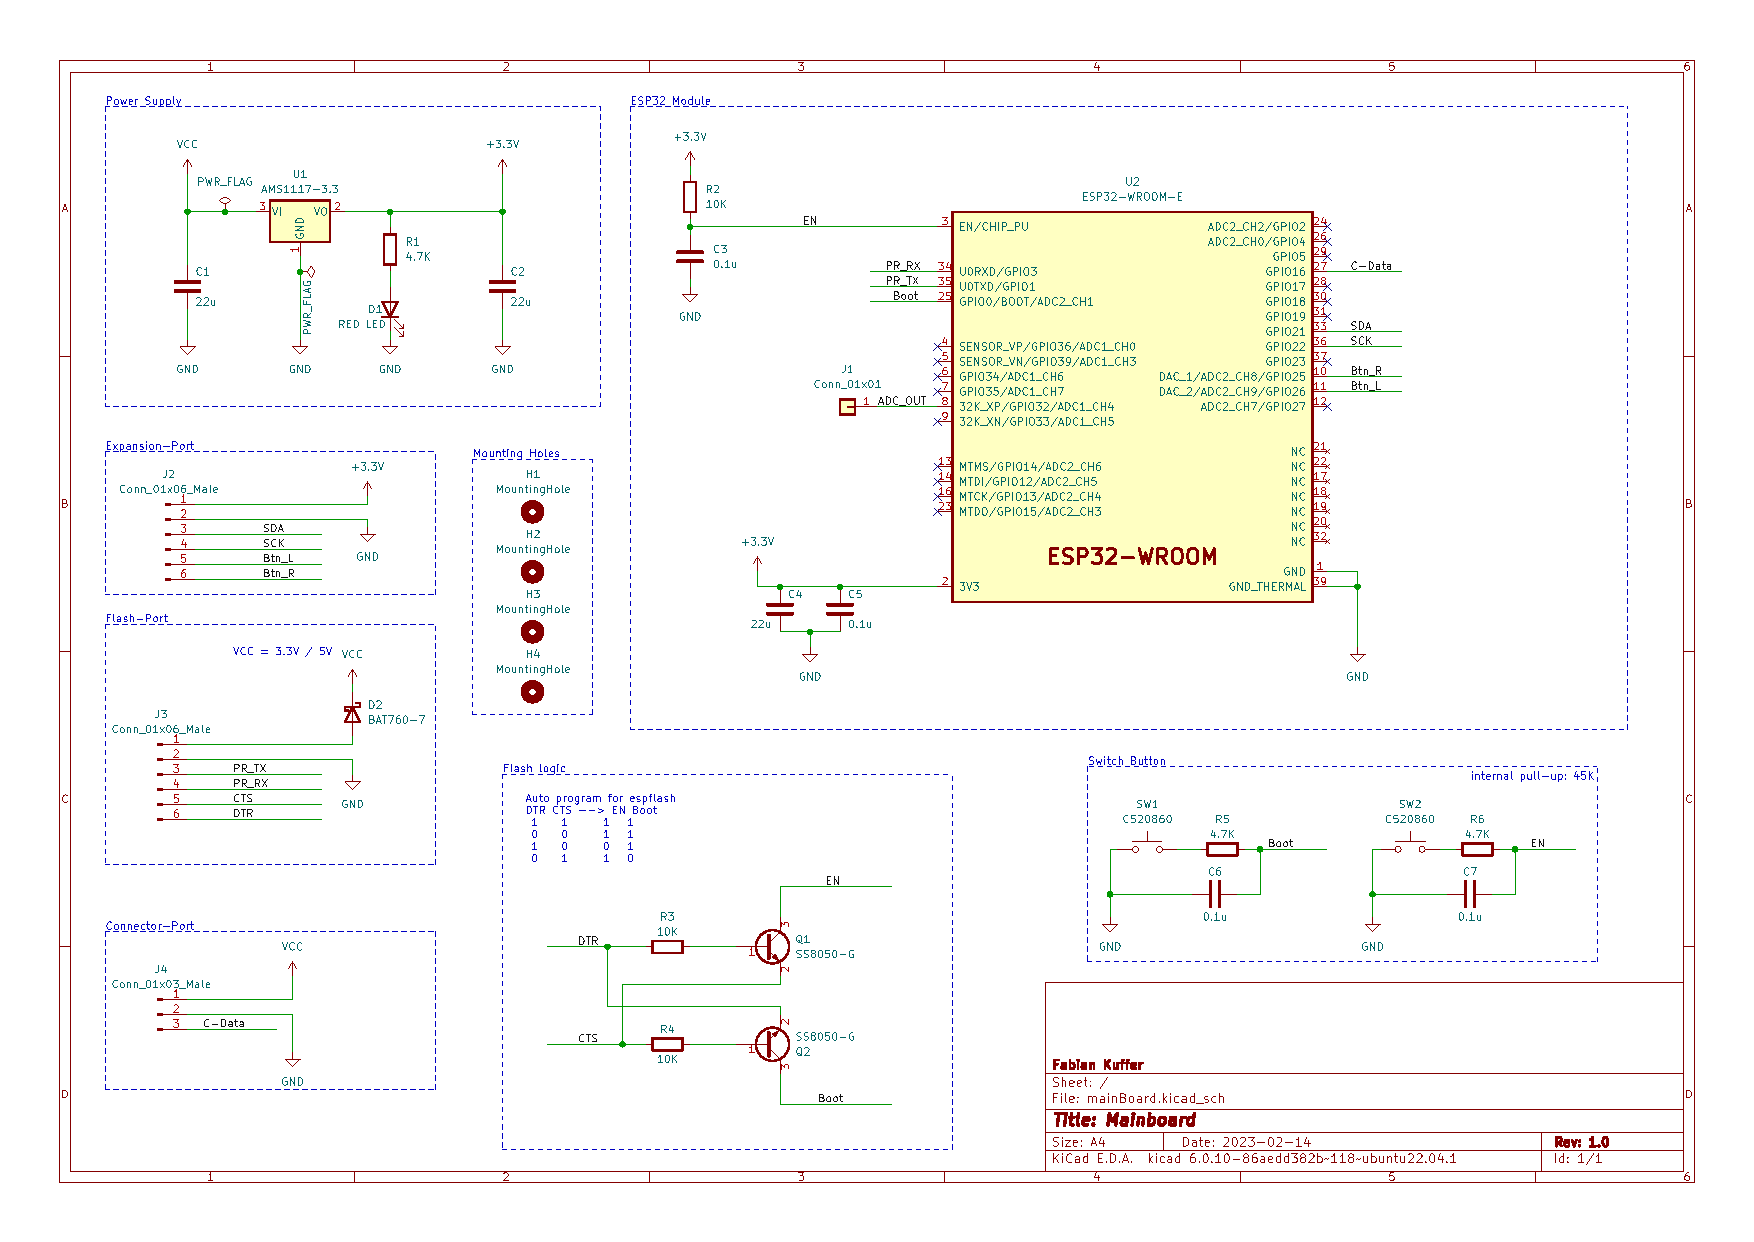
\includegraphics[width=0.73\textheight,angle=90]{../PDFs/mainBoard.pdf}
    \caption{Schaltplan der Hauptplatine}
    \label{fig:mainPCB}
\end{figure}

\begin{figure}[H]
    \centering
    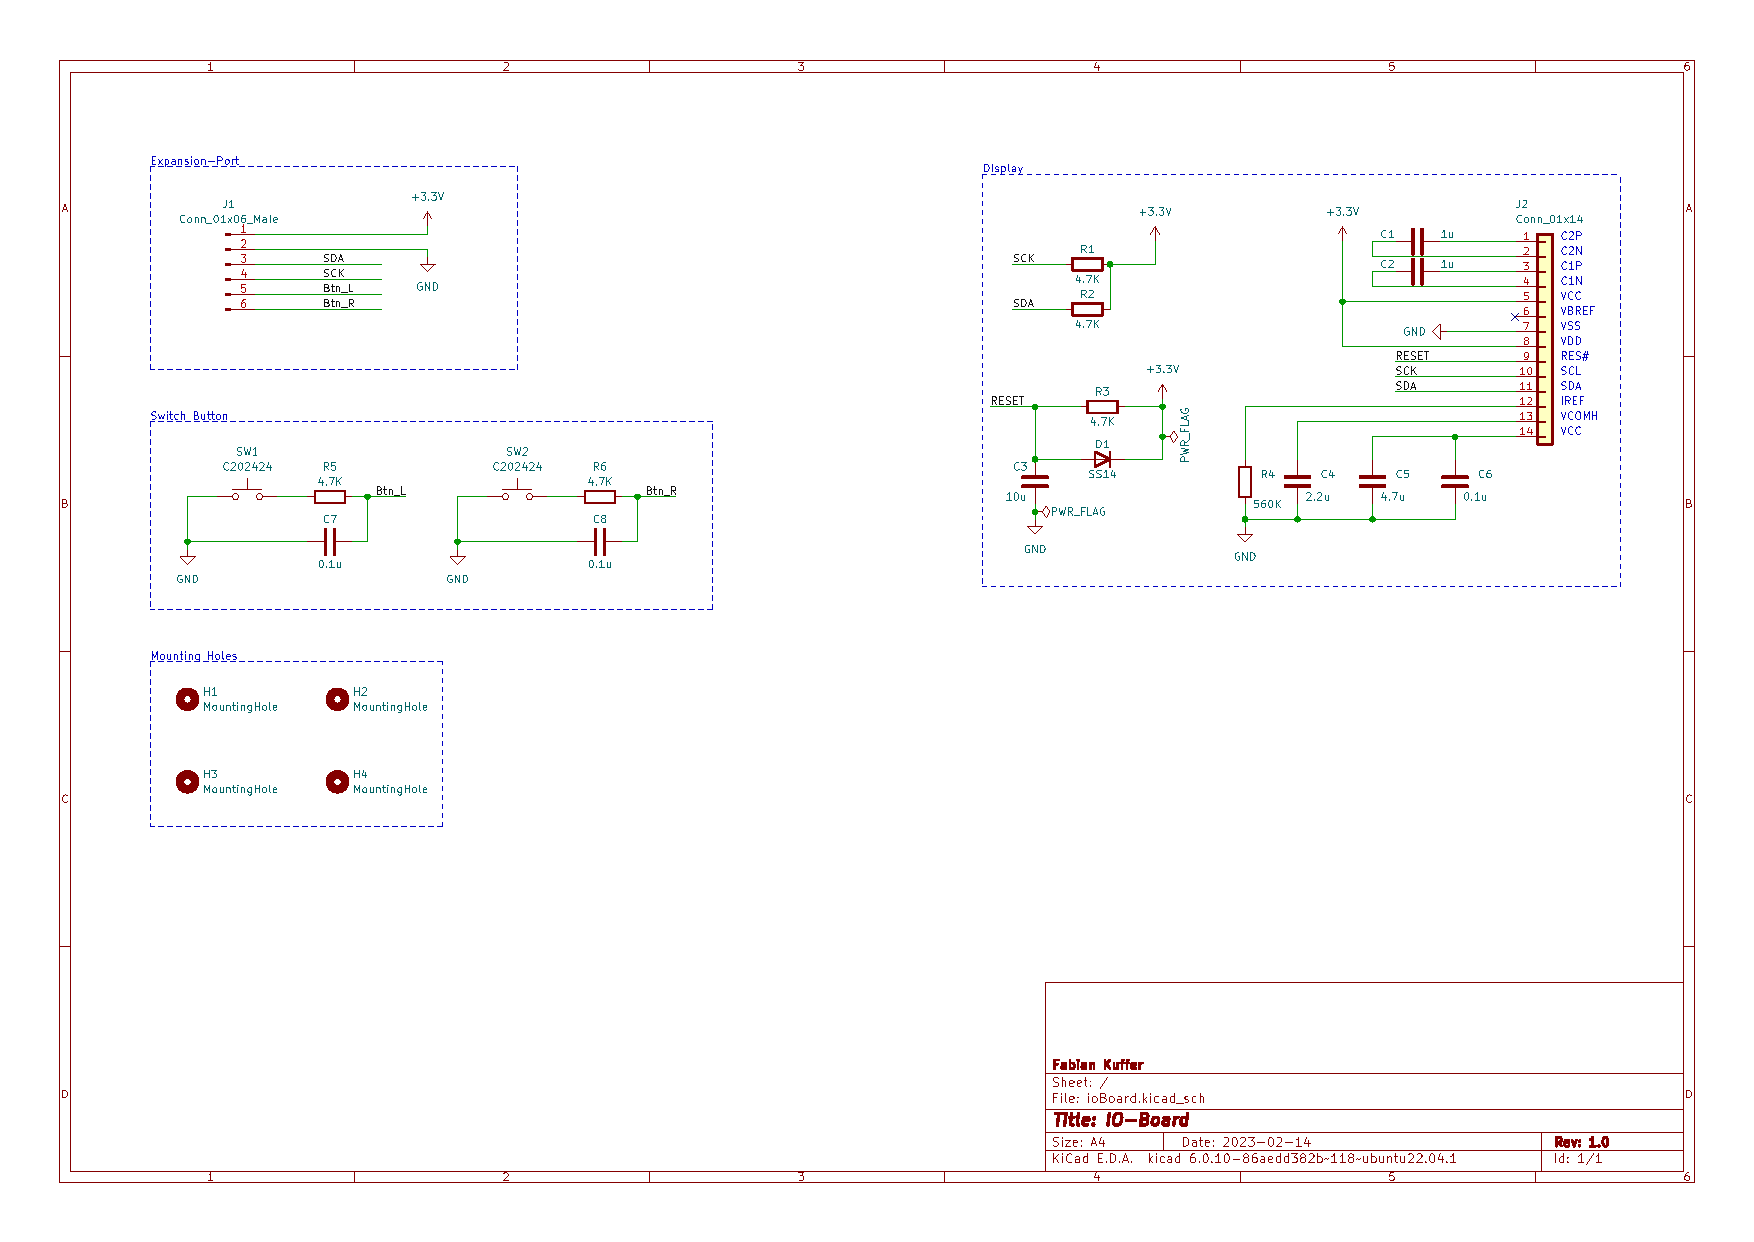
\includegraphics[width=0.9\textheight,angle=90]{../PDFs/ioBoard.pdf}
    \caption{Schaltplan für Ein- und Ausgabekomponenten}
    \label{fig:ioPCB}
\end{figure}

\begin{figure}[H]
    \centering
    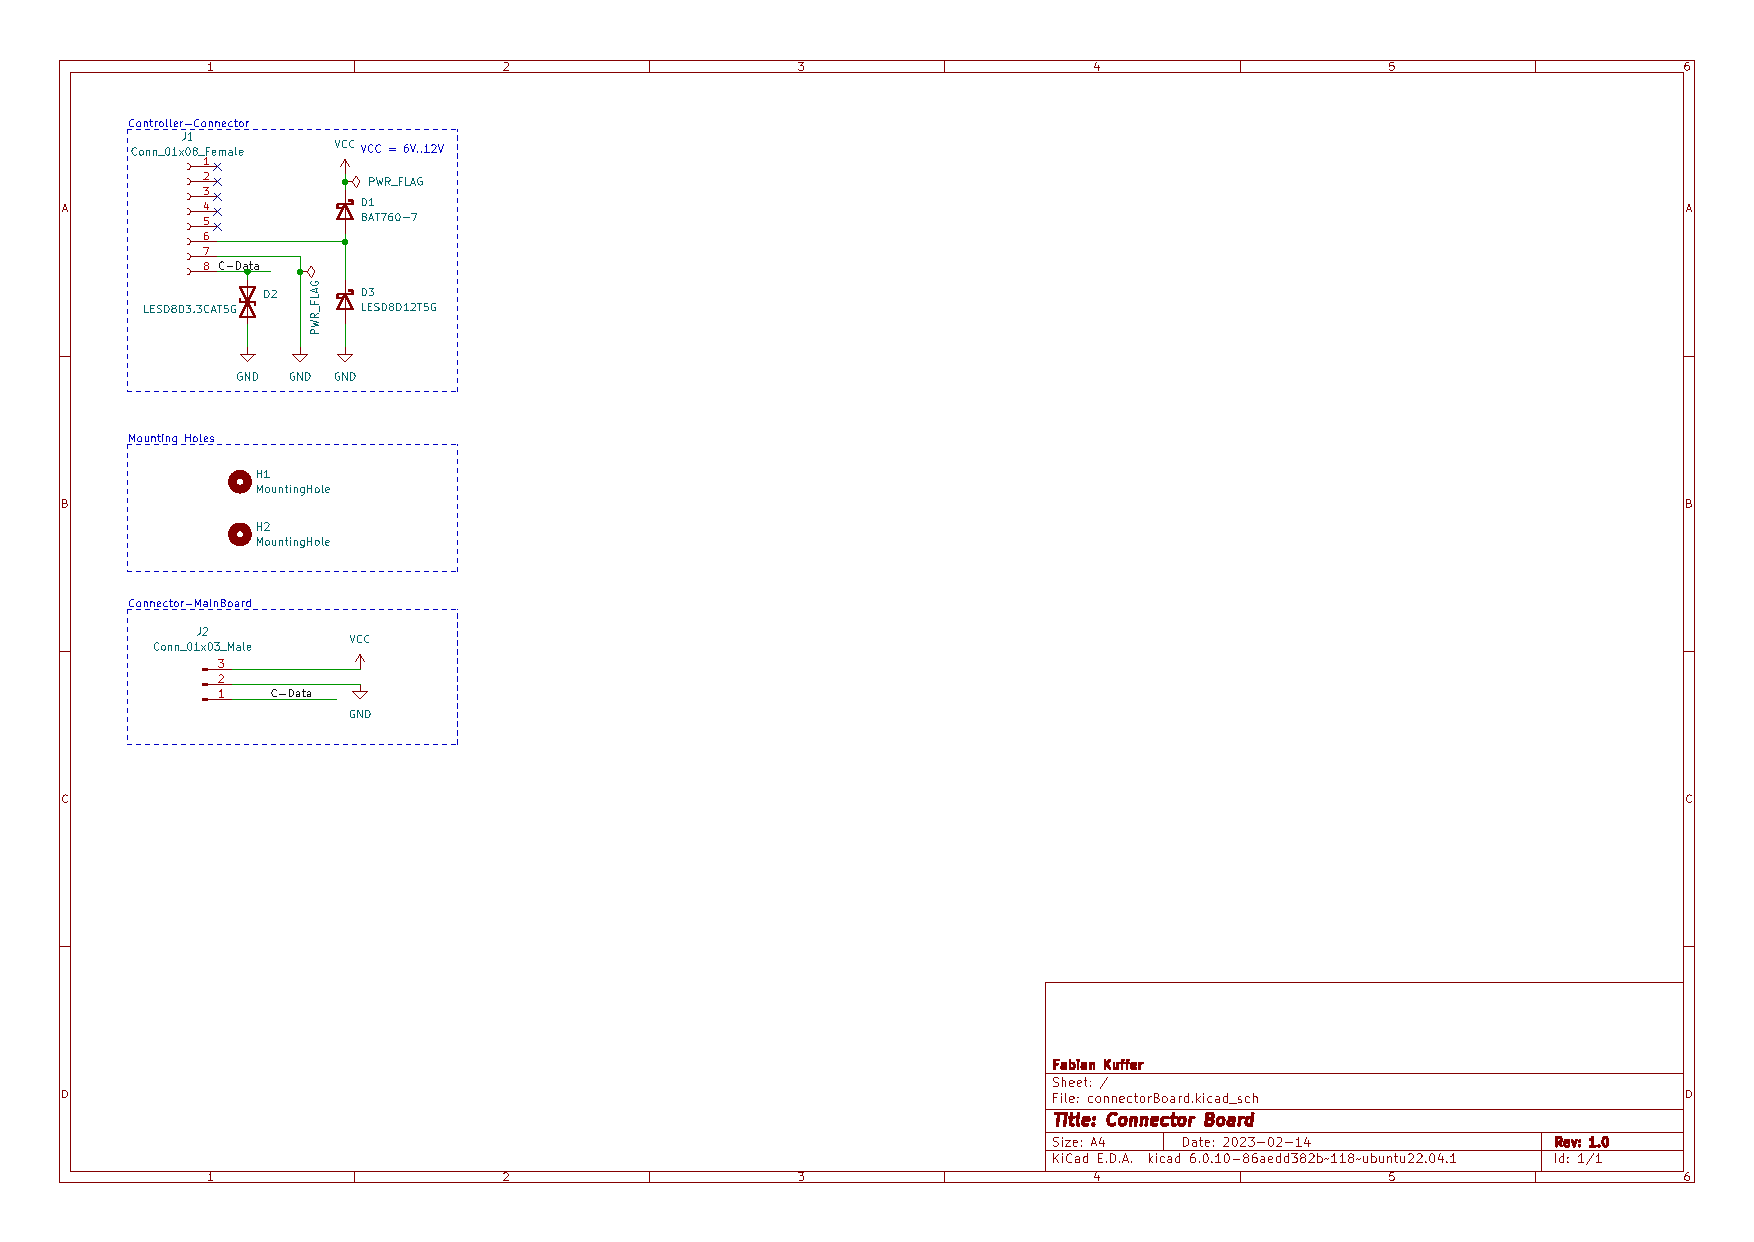
\includegraphics[width=0.9\textheight,angle=90]{../PDFs/connectorBoard.pdf}
    \caption{Schaltplan für die Verbindung zwischen Erweiterungsmodul und Multikopterfernsteuerung}
    \label{fig:connectorPCB}
\end{figure}

\section*{B. Explosionszeichnung des Gehäuses}
\begin{figure}[H]
    \centering
    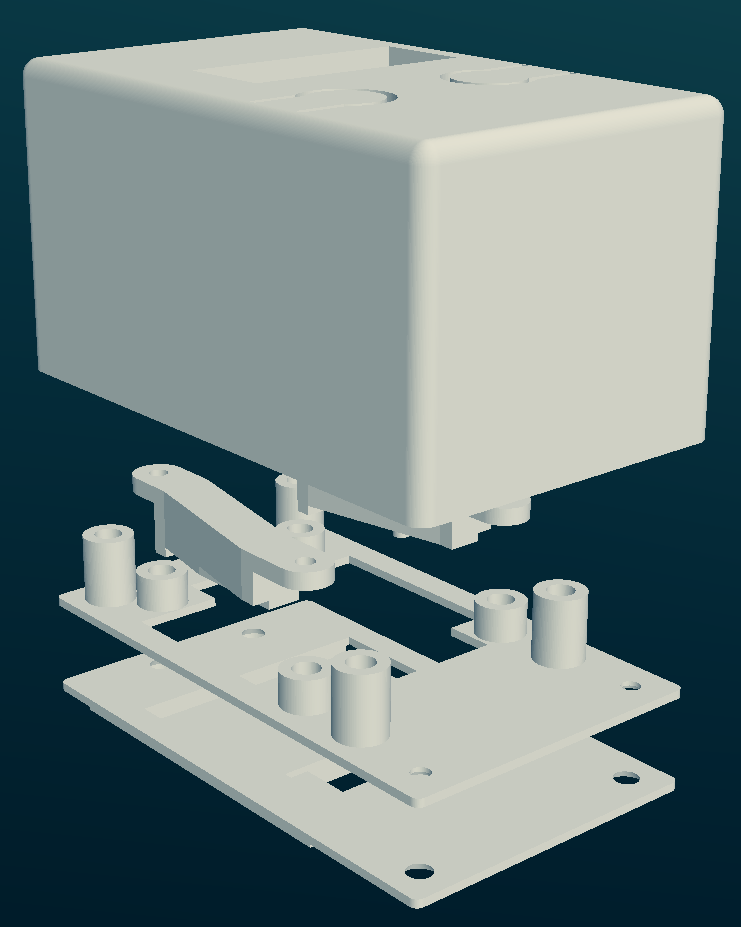
\includegraphics[height=0.5\textheight]{shellParts}
    \caption{Explosionszeichnung mit allen Modellen des Gehäuses}
    \label{fig:shellPartsExplosion}
\end{figure}